% ############### 2.1) OVERVIEW ####################

DREAM will be implemented using a Microservice Architecture and all the architectural choices reflect this main idea. We chose a microservice-oriented approach because it perfectly addresses the necessity of supporting a variety of different clients, the necessity of exposing an API for 3rd parties to consume and the necessity of guaranteeing high scalability and availability in a complex distributed system.

\begin{figure}[H]
	\centering
    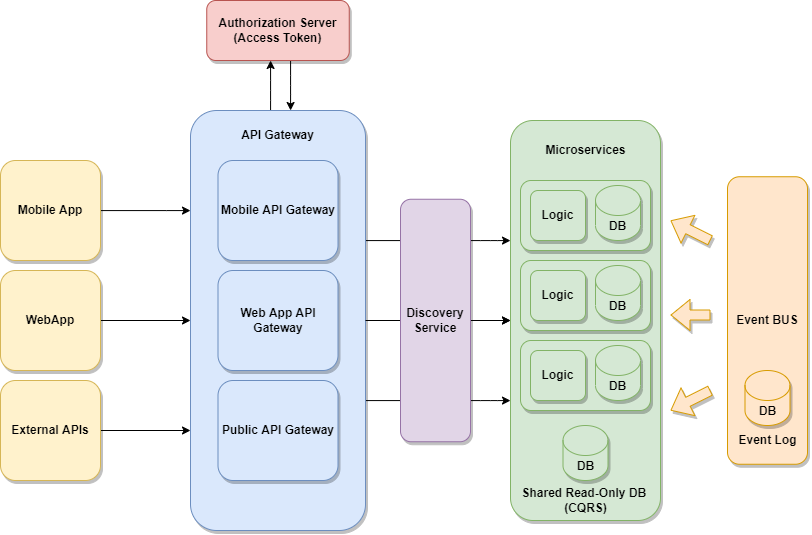
\includegraphics[scale=0.6]{Images/Architecture/Microservice Architecture Diagram.png}
	\caption{\label{fig:microservice_architecture}High-level Microservice Architecture}
\end{figure}

The system is logically divided in three high-level layers:
\begin{itemize} 
    \item presentation layer: it manages the presentation logic and all the interactions with the end user
    \item application layer: it manages the business functions that the S2B must provide
    \item data layer: it manages the safe storage and the relative access to data
\end{itemize}

According to these principles, the final architecture follows the client-server paradigm and is organized in 4 tiers (described in section 2.3). 
\newline

There are two types of client: the web application and the mobile app. The former is a thin client since it offers only presentation functionalities and depends entirely from the server, which contains all the application business logic. However, the mobile app is a more thick client because it contains an internal database, in order to be more independent from the server.
\newline

Figure \ref{fig:microservice_architecture} provides a high-level idea of the structure of the system and the interactions between the components. More precise information will be given in the following sections.

The users can access the service through a web interface or a mobile application. From there, the API gateway contacts the Authorization Server in order to guarantee security across the platform. After the identity has been checked, the Discovery Service is called to know the exact location of the microservices involved. The user’s request is then redirected to the correct microservice in which the business application logic is implemented. 

Each microservice has its own database, according to Microservice Architecture standards, and they all communicate through an Event bus (more details about the patterns used to keep these fragmented databases organized can be found in section 2.6). Finally, the system can interact with third party APIs and datasets through the API gateway.
\newline

Important note: the API gateway, the Authorization server and the Discovery Service are supposed to run on replicated machines, since they represent a single point of failure and can cause many problems to the overall service if they fail.

Moreover, all the application modules (especially the microservices) are expected to be stateless, according to the REST standard definitions (more details in section 2.6).

All the components will be described in depth in the following sections.
